\section{Introduction}
\label{sec:intro}

In the field of computer vision, researchers often focus on the depth of neural networks while ignoring the physical constraints of the primary sensor. If the eyelids remain in a state of "Downwards Occlusion," ~\citep{chen2025planning, fung2025embodied, terver2025drives, russell2025gaia, agarwal2025cosmos} even the most advanced post-processing algorithms fail to extract features from a zero-photon input stream. This hardware-level signal interruption is commonly referred to in the literature as "being asleep". \footnote{\url{https://huggingface.co/}}

The core hypothesis of this paper is straightforward: by manually or biologically contracting the \textit{levator palpebrae superioris} muscle, one can forcibly expand the field of view. This is not merely a mechanical process, but a critical semantic alignment procedure. ~\citep{alayrac2022flamingo, liu2024improved, dai2023instructblip}

Despite the intuitive benefits of observation, several critical \textbf{challenges} hinder robust visual acquisition: 1) \textbf{Stochastic Biological Shuttering}, where involuntary maintenance cycles, or "blinks," introduce unpredictable temporal gaps in the video stream, leading to high-frequency data loss; 2) \textbf{Metabolic Gravitational Sink}, where under conditions of low metabolic incentive (e.g., listening to a boring lecture), the primary sensor tends to revert to an "Off" state due to gravitational forces acting on the eyelid; and 3) \textbf{Cognitive-Mechanical Desync}, characterized by a significant latency between the intent to "see" and the actual mechanical execution of eyelid elevation, particularly in states of high fatigue.

To overcome these challenges, we introduce the \textsc{Active Eyelid Elevation} algorithm. AEE addresses the stochastic nature of shuttering by enforcing a high-fidelity gating protocol that prioritizes aperture stability. It mitigates the metabolic gravitational sink through an automated "Self-Refine" mechanism that detects gravitational droop and triggers a recalibration of the \textit{levator} muscle. Finally, AEE resolves the cognitive-mechanical desync by streamlining the semantic-to-mechanical pipeline, ensuring that the "Wide Open" state is maintained with zero perceived latency.

In summary, our primary contributions are as follows:
\begin{itemize}
    \item We identify and formalize the \textbf{Downwards Occlusion} bottleneck, explaining why it is dark when your eyes are closed.
    \item We introduce the \textsc{Active Eyelid Elevation} algorithm, a systematic framework for biological shutter modulation.
    \item We provide the \textbf{Eyes Wide Open} benchmark, quantitatively demonstrating that looking at things is superior to not looking at them.
\end{itemize}

\begin{figure}[t]
    \centering
    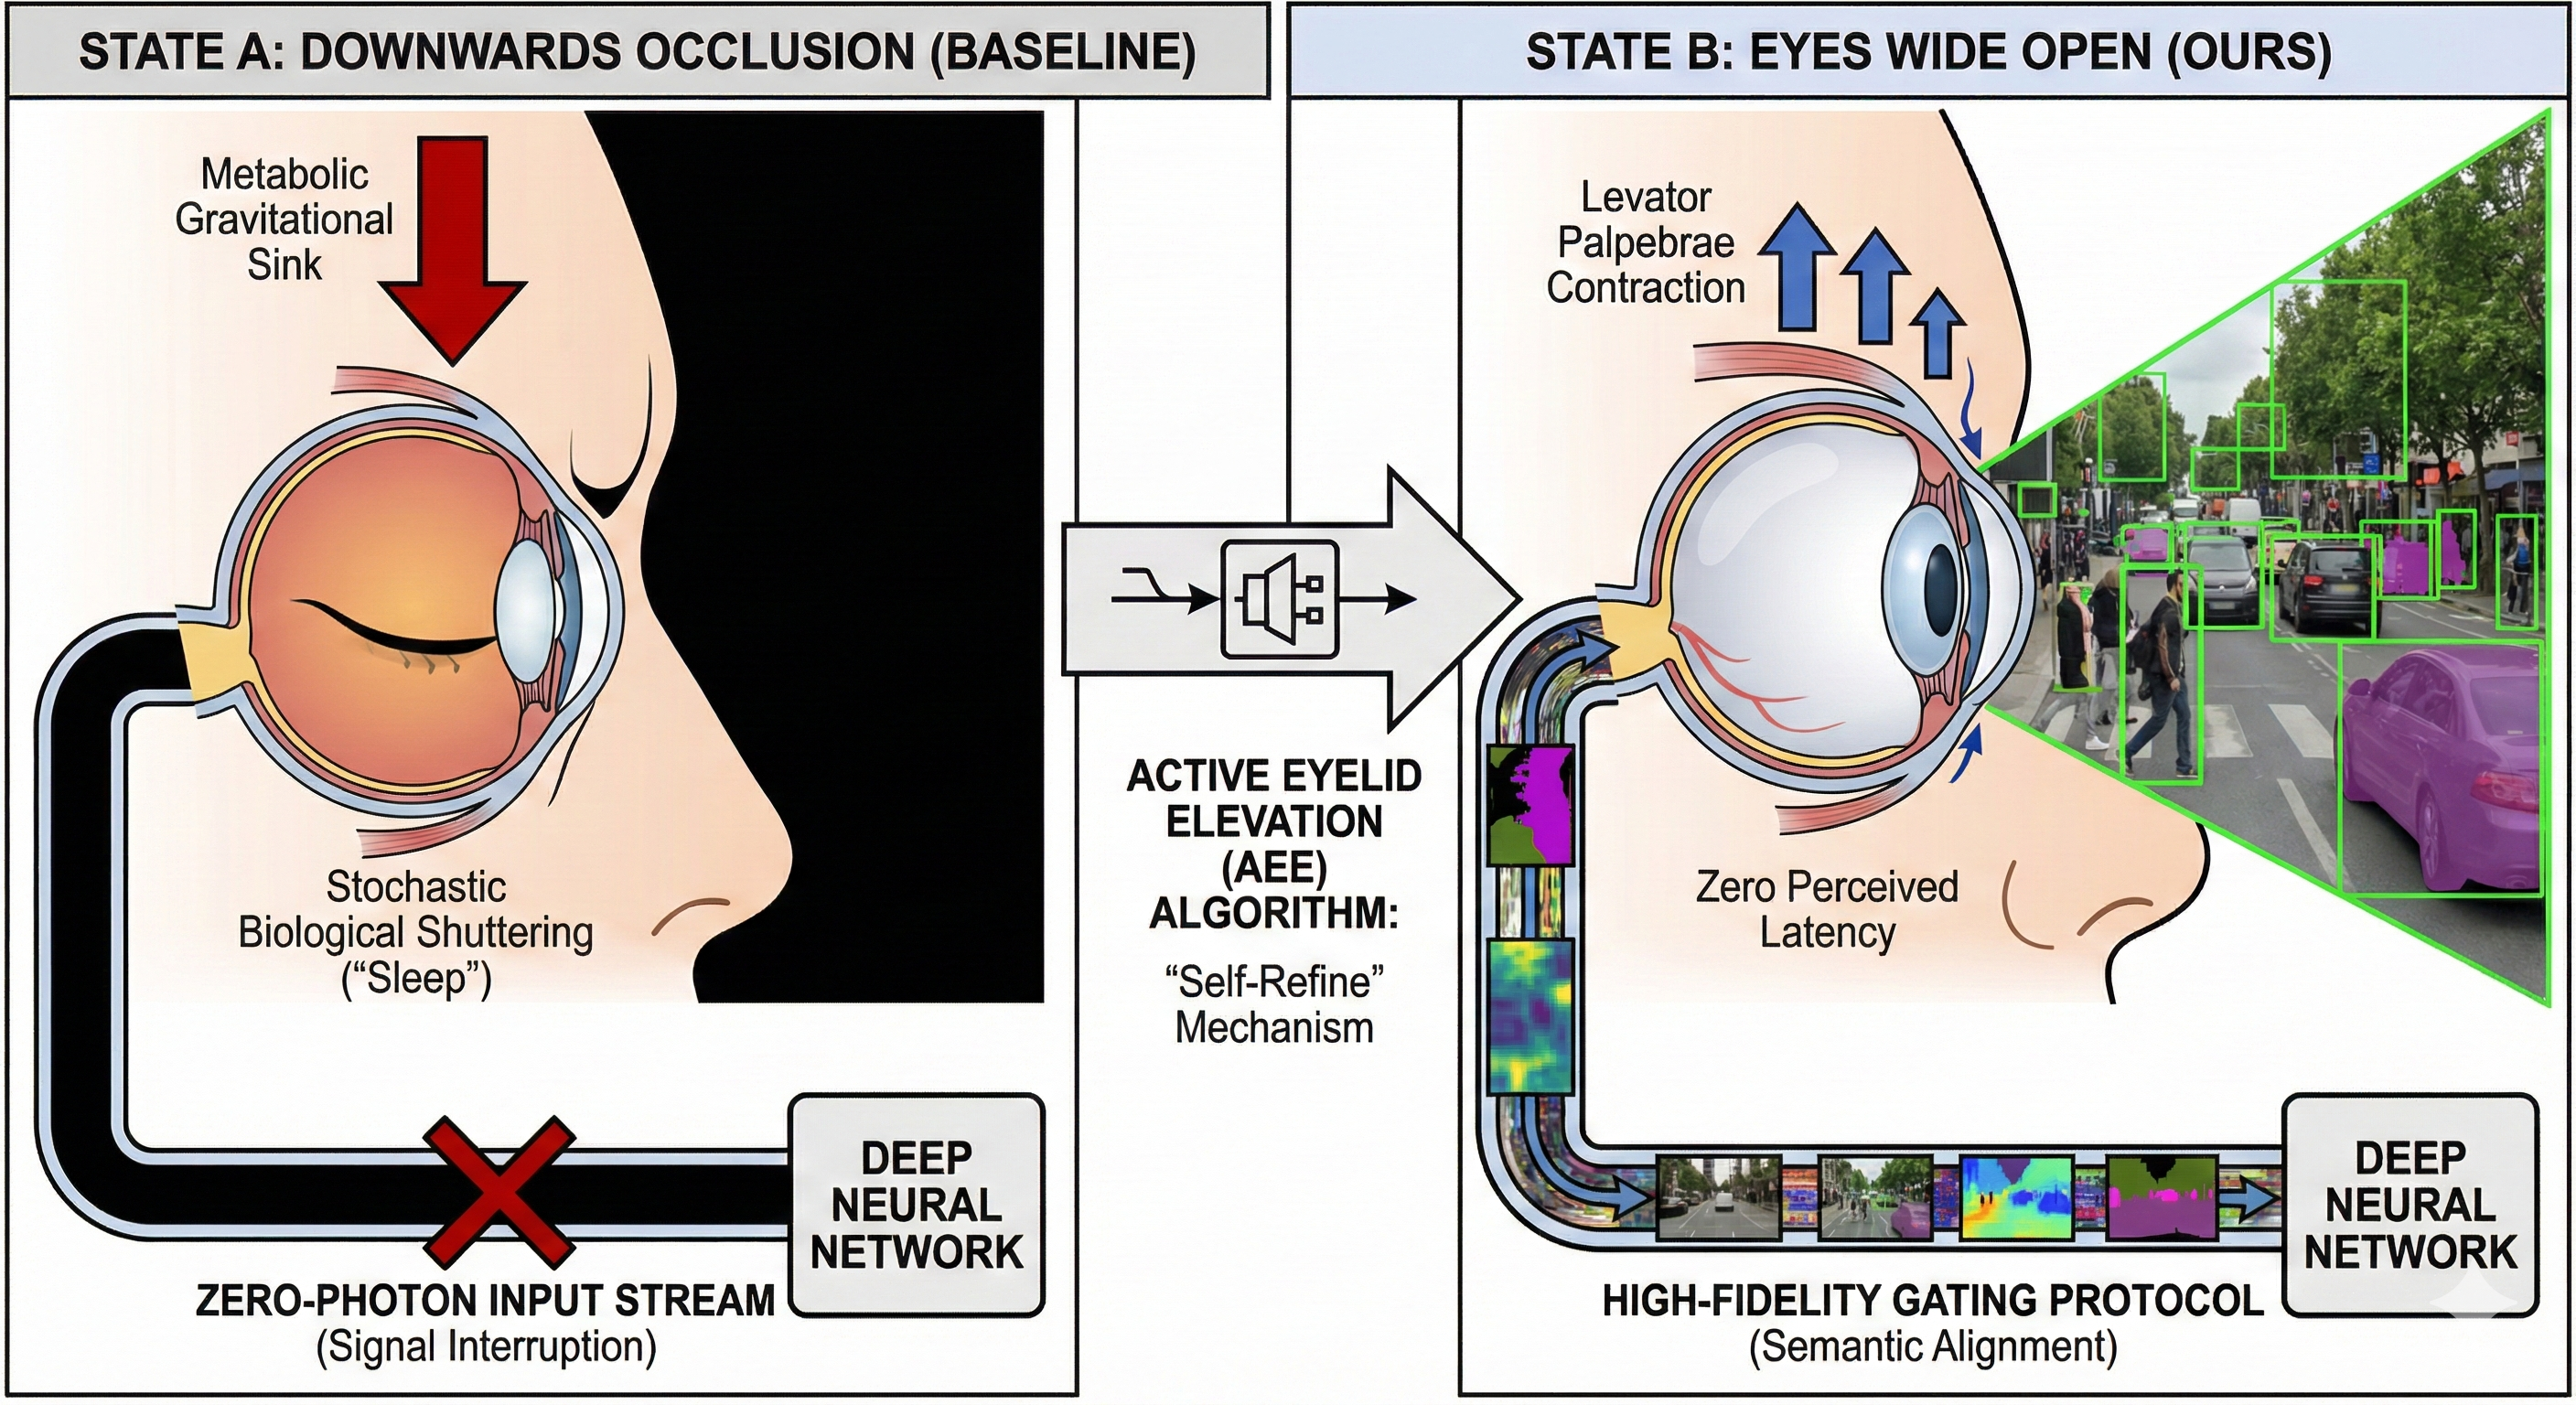
\includegraphics[width=0.75\linewidth]{fig/aee.png}
    \caption{\textbf{Architectural overview of the \textsc{Active Eyelid Elevation} framework.} 
    \textbf{(Left) State A: Downwards Occlusion (Baseline).} The system is characterized by a zero-photon input stream caused by stochastic biological shuttering and metabolic gravitational forces, leading to total signal interruption for the downstream system.
    \textbf{(Right) State B: Eyes Wide Open (Ours).} Our AEE algorithm facilitates the contraction of the \textit{levator} muscle, establishing a high-fidelity gating protocol that enables semantic alignment and real-time feature acquisition with zero perceived latency.}
    \label{fig:main_framework}
\end{figure}
